\documentclass[article,twocolumn]{memoir}
\usepackage[utf8]{inputenc}
\usepackage{psfrag}
\usepackage{hyperref}
\usepackage{color}
\usepackage[]{graphicx}

\graphicspath{{../figures/other/}{../figures/generated/}}


\title{Using Theatre to Fight HIV/AIDS in Mozambique}
\author{Rita Reis and Luis Pedro Coelho}

\bibliographystyle{alpha}
%\bibliographystyle{plain}
\pagestyle{Ruled}

\aliaspagestyle{chapter}{Ruled}
\makeatletter
\if@twoside
	\makeoddhead{Ruled}{}{}{\scshape\rightmark}
	\makeevenhead{Ruled}{\scshape\leftmark}{}{}
	\makeevenfoot{Ruled}{\pagenumberfont\thepage}{}{}
	\makeoddfoot{Ruled}{}{}{\pagenumberfont\thepage}
	% Put section number on top
	\def\sectionmark#1{\markright{#1 (\thesection)}}
	\def\chaptermark#1{\markboth{#1}{#1}}
	\renewcommand*{\bibmark}{\markboth{\bibname}{\bibname}} % I don't like empty headings!
\else

	% Put section number on top
	\def\sectionmark#1{\markright{#1 (\thesection)}}
	\def\chaptermark#1{\markright{#1 (\thechapter)}}

	\makeoddhead{Ruled}{}{}{\scshape\rightmark}
	\makeevenhead{Ruled}{}{}{\scshape\rightmark}
	\makeevenfoot{Ruled}{}{}{\pagenumberfont\thepage}
	\makeoddfoot{Ruled}{}{}{\pagenumberfont\thepage}
	\renewcommand*{\bibmark}{\markright{\bibname}} % I don't like empty headings!


\fi
\makeatother

%Change fonts: Page number sans-serif (much cleaner than the roman version)
\def\pagenumberfont{\sffamily}
% Change fonts: Section headers Sans-Serif:
\setsecheadstyle{\Large\sffamily\raggedright}
\setsubsecheadstyle{\large\sffamily\raggedright}
\setsubsubsecheadstyle{\normalsize\sffamily\raggedright}

% Title
\date{}
\pretitle{\LARGE\sffamily}
\posttitle{\par\vspace{4ex}}
\preauthor{\large\sffamily\hspace{1cm}}
\postauthor{\par\vspace{3ex}}
\predate{\small\sffamily\hspace{1cm}rreis@pointpark.edu and lpc@cmu.edu}
\postdate{\par\vspace{2cm}}
\copypagestyle{title}{plain}
\makeoddfoot{title}{}{}{}
\makeevenfoot{title}{}{}{}

\renewcommand{\abstractnamefont}{\sffamily}
\renewcommand{\abstracttextfont}{}
\renewcommand{\absnamepos}{flushleft}


\makechapterstyle{mestrado}{% Originally ``AlexanderGrebenkov'', adapted
\renewcommand{\chapterheadstart}{\goodbreak\vspace{\beforechapskip}}
\renewcommand{\chapnamefont}{\normalfont\Large\scshape}
\renewcommand{\chapnumfont}{\normalfont\Large\scshape}
\renewcommand{\chaptitlefont}{\normalfont\Large\scshape}
\renewcommand{\printchaptername}{}
\renewcommand{\chapternamenum}{}
\renewcommand{\printchapternum}{\normalfont\Large\scshape\S\thechapter}
\renewcommand{\afterchapternum}{\hspace{1em}}
\renewcommand{\afterchaptertitle}{\par\nobreak\vspace{-.9em}\moveright 6pt\vbox to 1pt{\hrule width .32\textwidth}\nobreak\vskip\afterchapskip\nobreak}
}
\chapterstyle{mestrado}

\begin{document}

\maketitle

\chapter{Introduction}

In July 2010, we worked with Kufunana, a non-profit organization in Mozambique,
which uses theatre, particularly theatre of the oppressed, to raise awareness
of HIV/AIDS issues. We directed a show with the actors of the association, a
show we developed collaboratively, inspired by Arthur Schnitzler's play ``La
Ronde.'' We also took the opportunity to talk to the members of Kufunana and to
interview them about their work.

In Mozambique, particularly in the region we were in, the Sofala province, HIV
is a major issue, with infection rates being approximately~20\%.

In Mozambican society, theatre is regularly used by many groups of local
volunteers to communicate social messages. Kufunana is one of the best known
groups in this area, but it is representative of a wider phenomenon.

We will present and discuss both the work we did with them and what we learned
from them through both discussions and formal interviews.

\chapter{Kufunana's Work}

Through structured interviews\footnote{We are making some of the videos
available, with English subtitles, online at: http://beiraproject.org.} and
informal discussions with the members of Kufunana we were able to gather
information on their actions in the social sphere.

Kufunana is a cultural organization that focuses on HIV/AIDS. Their main
artistic focus is theatrical, but they also have musicians, plastic artists,
and artisans. All of their members have been tested for HIV and most of them are
positive.

They often use theatre of the oppressed techniques in places around the city to
raise awareness on voluntary HIV testing (or sometimes other issues). They will
perform in markets, squares, discos, but also for private companies who hire
them to come and perform pieces on voluntary testing for their workers. This is
actually one of their main sources of income (which supports their
not-for-profit activities). Companies have now recognized that keeping their
employees in good health is in their best interests and that theatrical
representations are very effective towards that goal.

Their work starts with a short prepared play on HIV/AIDS, but leads to a wider
discussion of the issues using theatre of the oppressed techniques to draw in
audience participation. The workers often have the opportunity to get tested
immediately and to receive counseling (the results are confidential, of
course).

Additionally, Kufunana often travels to the country-side to do their work.
Their typical approach is to combine theatrical performances, theatre of the
oppressed, pure entertainment, and discussions. By renting a space such as a
local bar or discothèque, they attract a young crowd who comes for the music
and the entertainment. However, the entertainment is not empty entertainment
and the evening is be punctuated by other discussion events. And, as with the
theatrical presentations, even the music performed or played during the events
that Kufunana organizes will often be around the themes of HIV/AIDS. Thus, the
cultural aspect serves both to atract audience (very few people would show up
if all they advertised was debate) and also as a platform to discuss the
issues.

In our interviews, the members of Kufunana often blamed ``ignorance as well as
lack of knowledge.'' We realized that they would employ the word ``ignorance''
(actually, the Portuguese equivalent, \textit{ignor\^{a}ncia}, which, in
European Portuguese has the same meaning as the English word) to mean
``choosing to ignore the facts even if one knows them.'' This is one
justification for using theatre for social goals. It is not only that a
performance can attract more audience than a lecture, it can lead to reflection
on behavior and behavioral change. A lecture can only impart knowledge and lack
of factual knowledge is not the only obstacle in the way of change.
Empathizing with a character or witnessing a situation as a spectator can
create a strong reaction leading to behavioral changes in the audience members.

\chapter{A Rede (The Network)}

La Ronde by Arthur Schnitzler is a play from 1900, set in Vienna. It is
structured as a series of encounters between a man and a woman. Character~1
meets (and has sex) with character~2, character~2 meets (and has sex) with
character~3, character~3 meets (and has sex) with character~4 and so on. This
continues until character~10 has a sexual meeting with the first character,
closing the loop (hence the name of the play). In each scene, the actual sexual
act is represented by a short blackout. The characters are representative of
types from all the social classes of the \textit{fin de siecle} Austrian
society, such as: prostitutes, soldiers, noblemen\ldots While watching these
sexual encounters, the spectators witness the seduction and power games that
sex can trigger and are able to observe a part of society that is often
invisible.

One of the readings of the play is that the subtext is the transmission of
Syphilis, the venereal disease of the time, through society. After having
learned about Mozambican society through discussions with the members of
Kufunana and others, we were reminded of Schnitzler's play. We imagined we
could adapt it to address the spread of HIV, the relevant sexually transmitted
disease of today, in Mozambique and around the world.

We described the basic outline of Schnitzler's La Ronde to the actors of
Kufunana. We made it clear that we did not intend to perform this European play
(even if it is a marvelous play), but to use it as the conceptual foundation.
Some of the members of Kufunana related it to a recent concerted effort by
HIV-related NGOs to make people aware of the sexual networks of which they are
a part of. Thus the idea developed from the circle to the network.

We started work to develop these ideas into a show. All of our scenes emerged
organically through improvisation with the actors. Actors were not assigned
roles at this stage and some situations (for example, teacher and female
student exchanging sex for grades) were developed by several actor couples. The
actors had a mandate to explore themes related to sexual encounters in
Mozambique. We were looking for character types that would be recognizable to
the Mozambican audience.

We used the characters of La Ronde as an inspiration, and tried to find
Mozambican equivalents to the Austrian fin de sci\'{e}cle types. Working from
the actors' propositions we where able to find equivalents to practically all
of Schnitzler's characters. And where surprised to notice how easily those
types operate in such different settings.

In addition to on-stage work, we had discussions with the actors about whether
the piece represented Mozambican society and, if not, what was missing. For
example, at one point, we realized that we had a rich man, but no politically
powerful figures (particularly important in a society so marred by corruption).
This discussion led us to add a member of parliament.

We had an imbalance in distribution, with more male actors than female actors.
We had not chosen the actors to work with, but worked with those that were
interested. Partially for this reason, but also to introduce outside observers
that could comment on the actions of the other characters, we introduced what
we called a ``Greek chorus of drunkards.'' Their goals and actions were be
similar to the Greek chorus of classical tragedies: to foreshadow events, to
tell the back story, and to provide the \textit{vox popolis}. However, to
introduce a traditional Greek chorus would be a completely foreign element to
Mozambican culture and would not resonate with the audience. Therefore, we had
the men of the chorus sit at a bar, on one end of the stage, drinking and
talking about the main actions between the scenes.  Their inebriation served as
the naturalistic justification for their frankness about everyone in the
community.

To represent two of the sexual scenes, we developed a dance representation of
the sexual transmission of HIV. In one of these scenes, there is viral
transmission. In the other one, between the Prostitute and a Truck-Driver, the
Prostitute, who always protects herself, wears a condom. Thus, she is able to
fight off the infection. Again, even if the scene is meaningful artistically and
socially, it emerged from discussions where we learned that, today, prostitutes
in Mozambique tend to protect themselves more frequently than other women. One
of the Prostitute's most resonating lines was: ``what do you think I am selling
here! I'm selling my body, not my health!'' The dance representations were
developed with the actors and set to traditional African drumming.

One of the main goals of Kufunana is to promote condom usage. That is why most
scenes we worked on include a negotiation around condom usage. One of the goals
was to portray various reactions to the suggestion of condom usage. After the
contamination dance, which was one of the first scenes of the show, the
audience knew that all the members of the network could potentially get
infected. Therefore, they understood that this negotiation is a matter of life
and death. One of the members of Kufunana, who is HIV-positive, once told us
how difficult those negotiations sometimes could be ``most of the time, the
girl won't understand that I actually want to protect her!''

\chapter{Discussion}

In summary, we used a collaborative effort to adapt a century old play about
\textit{fin de si\'{e}cle} Austria for the to modern day Mozambique. We chose
La Ronde because its themes find a parallel in Mozambican society.  As
outsiders, we brought this idea to the group, but let their responses
organically mold the show as we would be otherwise unable to create something
that spoke to a community with which we were unfamiliar. Although the content
was particular to the society we were working in, we think our working approach
would be useful in any community in which one is working as an outsider with
local actors. As a side effect of creating this show, we learned much about the
structure of Mozambican society, particularly its sexual economy, as depicted
by the actors on stage.

In Mozambique, sex is not often given for free, but in exchange for gifts or
money (even inside of stable relationships). One of the couples in the play, a
young man and woman, were set to represent an exchange-free relationship.
Although we were assured that this does happen in their society, at one point,
one of the actors had to resort to explaining to another the point of that
scene: "it's like in the movies, they are together for love, not for anything
else.''

We kept La Ronde's the scene structure. Almost all of the scenes are partner
scenes with a sexual encounter towards the end. We had characters from all
strata of society. Most of the characters in Schnitzler's play find a
correspondent in our version: the Teacher for the Poet, the Congressman and his
Wife for the Husband and his Young Wife, the Policeman for the Soldier\ldots
One character is present without any cultural adaptation, namely, the
Prostitute.

Artistically, the result is sometimes a mix of Western and local, for example
the danced scenes would not be out of place in a modern Western show, but they
were set to traditional African drumming. Another scene, set in a discotheque,
featured loud Mozambican pop, local music inspired by Western forms.

This type of creation process is also used by Western theatre groups, even
though it is not very frequent. But we would like to point out one of the main
differences between this collective creation and the ones we have been a part
of in the past, this is an oral experience. Written text is not one of the
steps of the process. Even though the plot and the main spoken lines stay the
same the actors continued to improvise text during the performances. We also
noted that, with the actors of Kufunana, there was little sense of artistic
property and actors were happy to let others take over the scene they had
created.

\chapter{Conclusions}

La Ronde is fecund starting material for theatre groups that want to raise
awareness on HIV/AIDS. It has a powerful structure that makes the audience
members realize that anyone can be infected. An adaptation of La Ronde depicts
the games of power and seduction that sexual encounters involve and the social
layers of society. Therefore, it can allow an interesting observation of the
society where the adaptation is made.

We have described our interactions with Kufunana and how they use theatre to
reach out. We have omitted their other activities as they would be beyond the
scope of this paper, but we will note that they perform many other services for
the community.

We described our work with them, which we believe can serve as a model for
working in any community to which one comes as an outsider. We brought our
inputs, our techniques, but we used them to start a discussion and then used
mainly improvisation on stage and discussion off stage to mold the show into
something that could be used to discuss the issues in that society.

We have learned a lot from this exchange. In Western countries, it is sometimes
said that theatre is a dead art. But for the members of Kufunana we worked
with, theatre is an essential vehicle to fight HIV/AIDS, a battle that concerns
the members of the association personally and that is vital for Mozambique.

The Network is still being performed by Kufunana, sometimes in full, but, most
of the time, excerpts are used during the theatre--music--debate events that
the association organizes to raise awareness on voluntary HIV testing.

\begin{figure*}[b]
\begin{center}
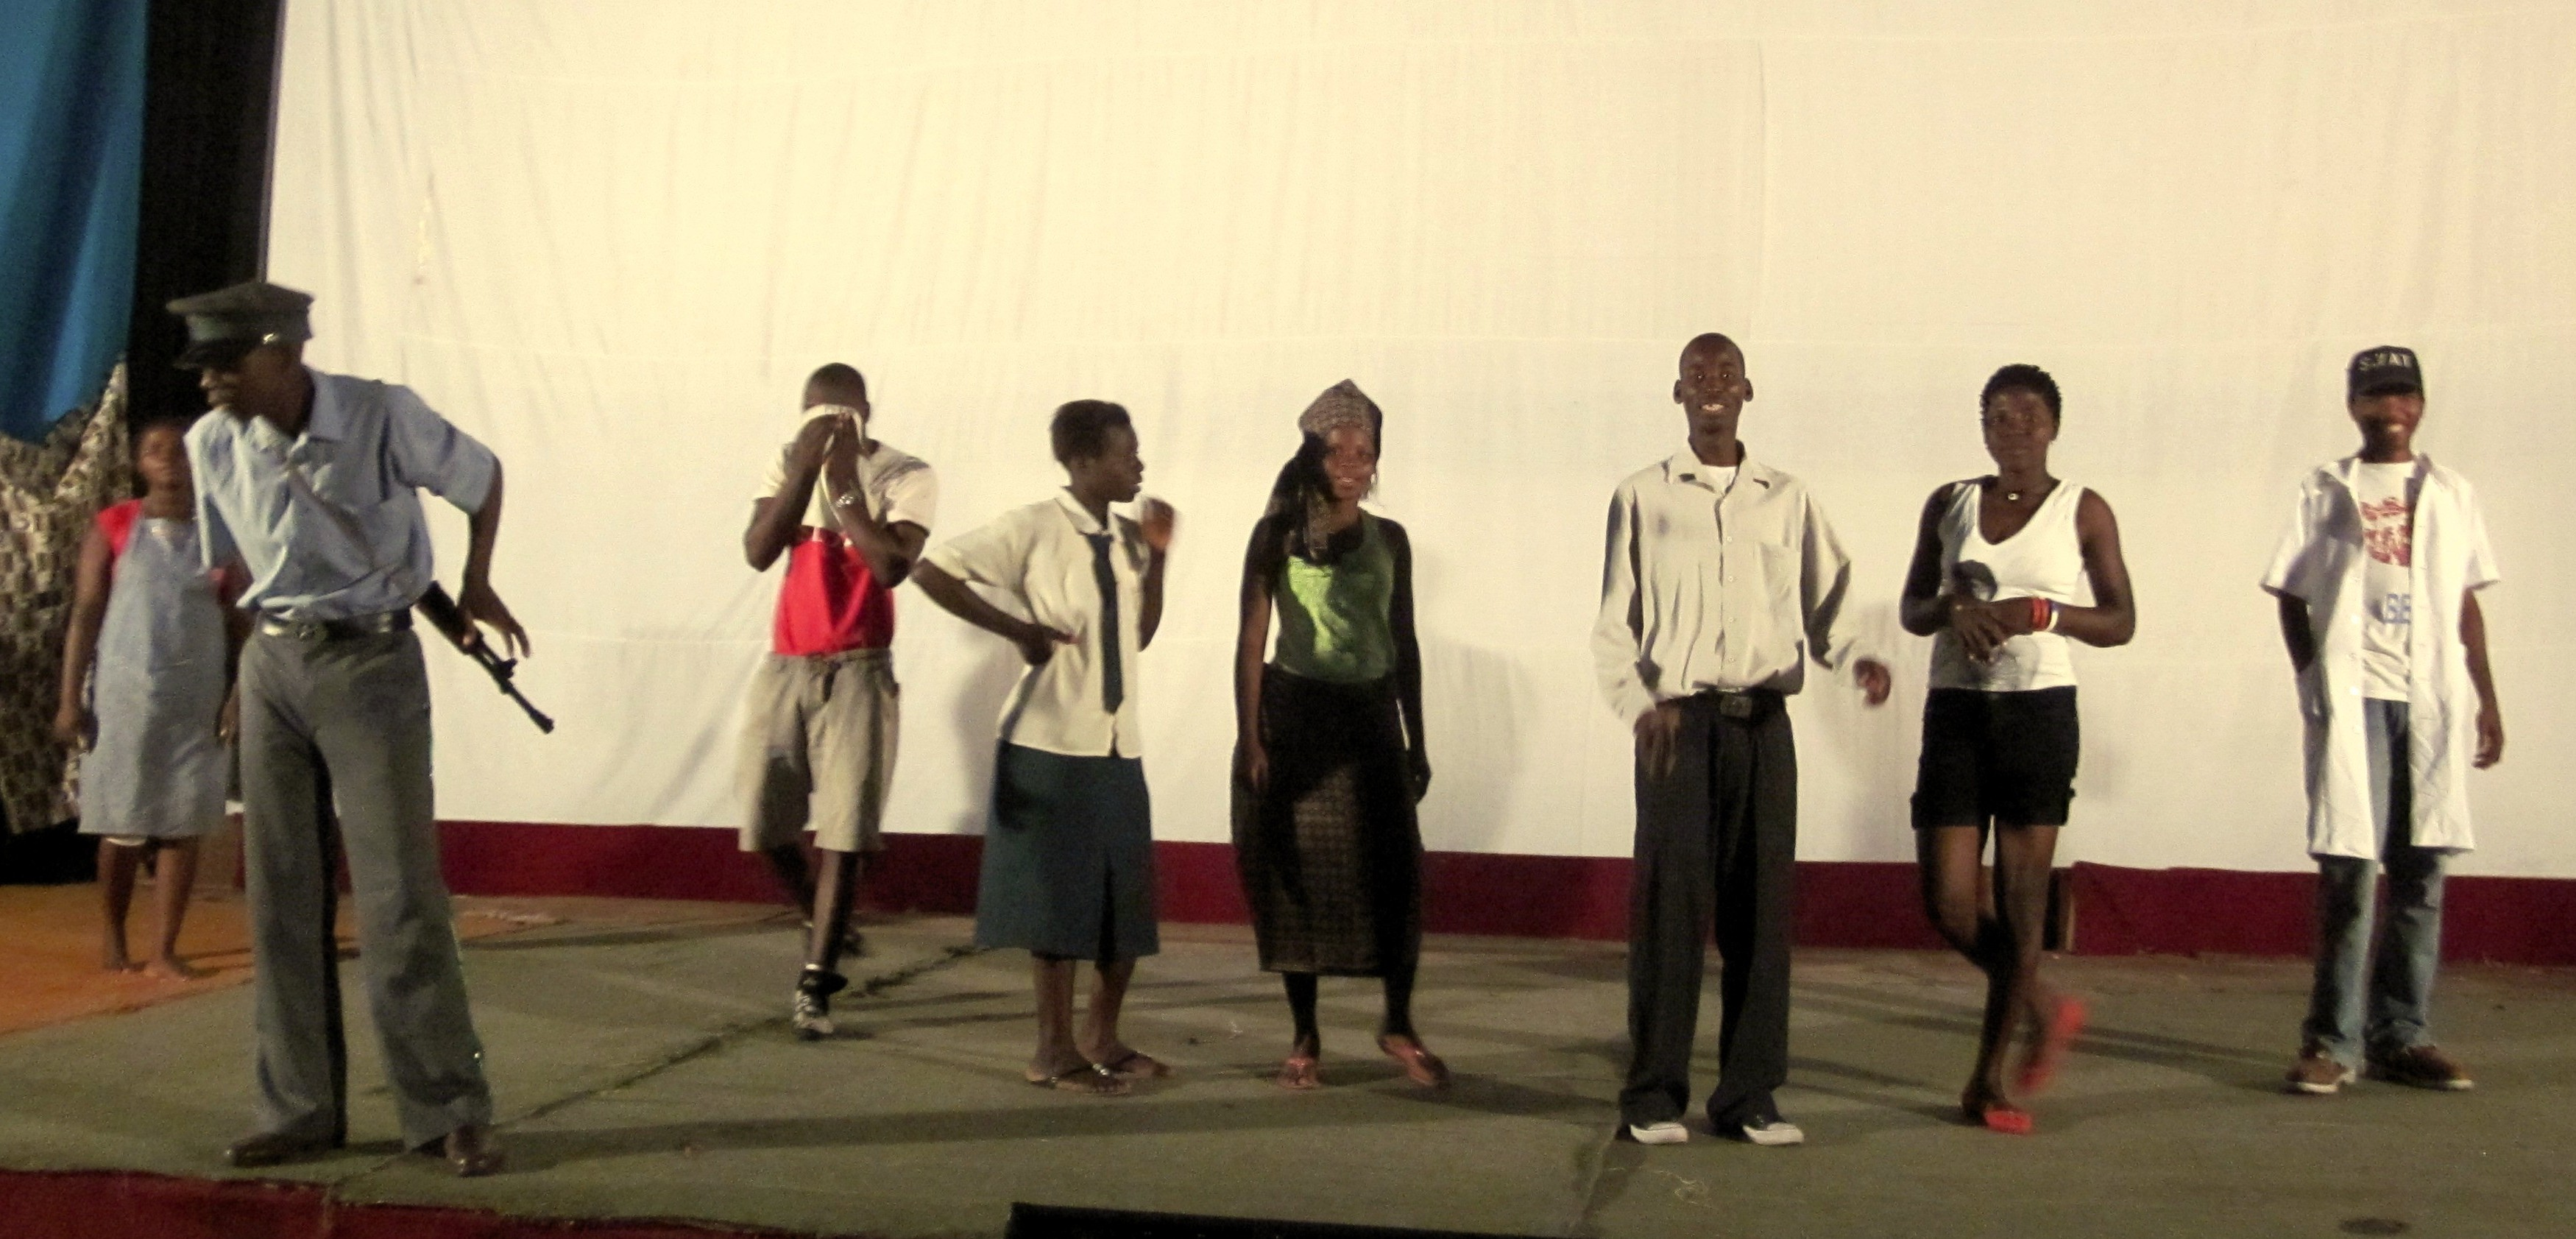
\includegraphics[width=.9\textwidth]{photographs/actors.jpg}
\end{center}
\caption{Actors, in costume, preparing for the show. Beira, Mozambique, July 2010.}
\label{fig:actors}
\end{figure*}


\begin{figure*}[b]
\begin{center}
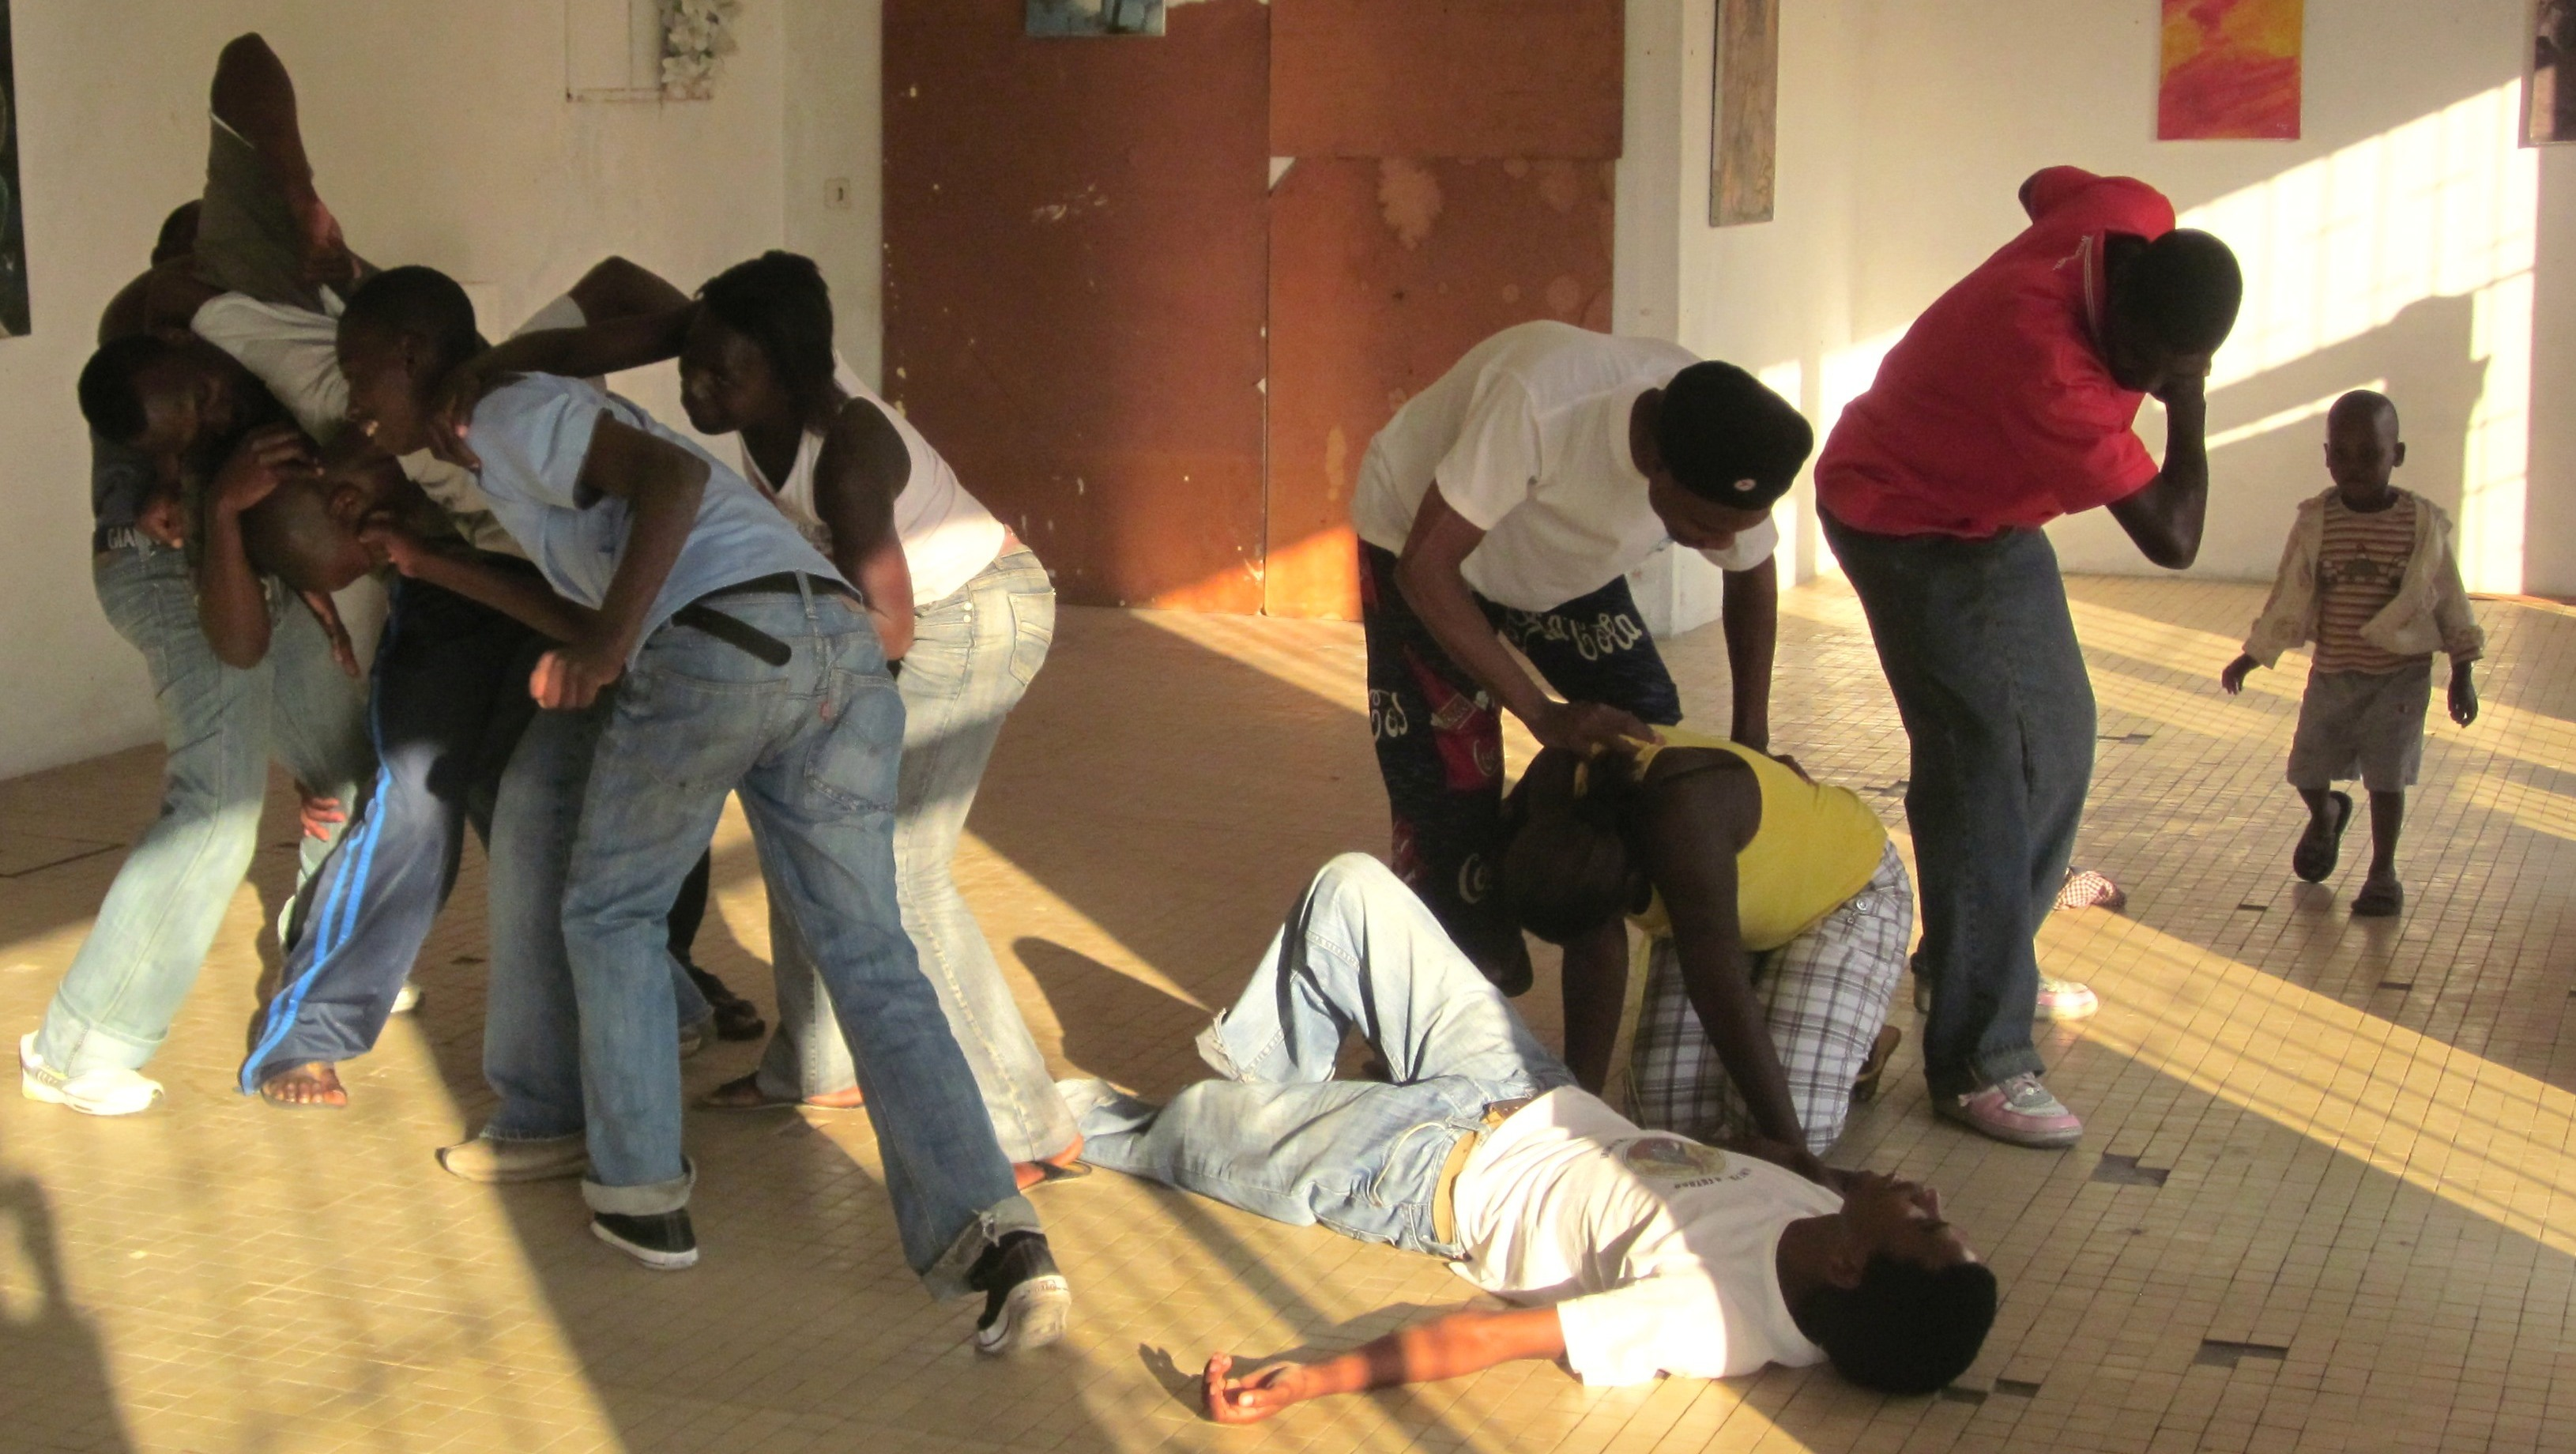
\includegraphics[width=.9\textwidth]{photographs/exercises.jpg}
\end{center}
\caption{Kufunana actors, during a movement exercise. Beira, Mozambique, July 2010.}
\label{fig:exercise}
\end{figure*}


\end{document}
